\documentclass[a4paper,12pt]{article}
\usepackage{graphicx}
\usepackage[utf8]{inputenc}  
\usepackage[T1]{fontenc}
\usepackage{gensymb}

\usepackage{helvet}%Police Arial
\renewcommand{\familydefault}{\sfdefault}

\usepackage[top = 1cm, bottom = 2cm, left = 1cm, right = 1cm]{geometry}
\usepackage{titlesec}
\setcounter{secnumdepth}{4}
\usepackage{xcolor}
\usepackage{amssymb} %double flèche de réaction
\usepackage{xtab}%tableau sur plusieurs pages
\usepackage{esvect}%grands vecteurs

 \usepackage[version=4]{mhchem} %equations chimiques

\usepackage{array}
\usepackage{chemfig}
\usepackage{multirow}
\usepackage{sectsty}
\usepackage{caption}
\usepackage{amsmath}
\usepackage{amssymb}
\usepackage[cal=boondoxo]{mathalfa} 
\usepackage{enumitem}
\usepackage{lastpage}
\usepackage{tcolorbox}
\usepackage{siunitx}
\usepackage{tikz}
\usepackage{multicol}%pour écrire sur deux colonnes où l'on veut
\sisetup{
    detect-all,
    output-decimal-marker={,},
    group-minimum-digits = 3,
    group-separator={~},
    number-unit-separator={~},
    inter-unit-product={~}
} %setup pour SIunitx
\usepackage{listings}%pour insérer le code python
\definecolor{codegreen}{rgb}{0,0.6,0}
\definecolor{codegray}{rgb}{0.5,0.5,0.5}
\definecolor{codepurple}{rgb}{0.58,0,0.82}
\definecolor{backcolour}{rgb}{0.95,0.95,0.92}

\lstdefinestyle{mystyle}{
    backgroundcolor=\color{backcolour},   
    commentstyle=\color{codegreen},
    keywordstyle=\color{magenta},
    numberstyle=\tiny\color{codegray},
    stringstyle=\color{codepurple},
    basicstyle=\ttfamily\footnotesize,
    breakatwhitespace=false,         
    breaklines=true,                 
    captionpos=b,                    
    keepspaces=true,                 
    numbers=left,                    
    numbersep=5pt,                  
    showspaces=false,                
    showstringspaces=false,
    showtabs=false,                  
    tabsize=2
}

\lstset{style=mystyle}

\graphicspath{ {/home/remy/Documents/Enseignement/2022/Tspe/C8/Ressources/} }

\sectionfont{\fontsize{14}{8}\selectfont}
\renewcommand{\thesection}{\arabic{section}.}
\renewcommand{\thesubsection}{\hspace{1cm}\alph{subsection}.}

\title{\vspace{-1cm}\large 
	\begin{tabular}{|>{\centering}m{5cm}|>{\centering}m{8cm}|>{\centering\arraybackslash}m{4cm}|}
	\hline
	Exercices & \textbf{\textsc{Équilibres acide-base}} &  Chapitre 8\\
	\hline
	\end{tabular}}
\date{}

\newpagestyle{mystyle}{%
\setfoot{}{\thepage\,$|$\,\pageref{LastPage}}{}
}
\renewpagestyle{plain}{%
\setfoot{}{\thepage\,$|$\,\pageref{LastPage}}{}
}

\pagestyle{mystyle}

\newenvironment{itemize*}%
  {\begin{itemize}[label=$-$]%
    \setlength{\itemsep}{0pt}%
    \setlength{\parskip}{0pt}}%
  {\end{itemize}}

\newenvironment{itemize**}%
  {\begin{itemize}[label=]%
    \setlength{\itemsep}{0pt}%
    \setlength{\parskip}{0pt}}%
  {\end{itemize}}
  
  
\begin{document}
\maketitle
\vspace{-2.5cm}

\section*{Exercice 1 : pH d'une solution d'acide fort}
L'acide chlorhydrique est un acide fort dans l'eau. Une solution $S$ de concentration en soluté apporté $c$ = \num{4,0e-2} \unit{\mole \per \liter} est préparée.
\begin{enumerate}
	\item Rappeler la définition d'un acide fort\\
	\textcolor{blue}{Un acide fort est un acide dont la dissociation dans l'eau est totale. La réaction mise en jeu sera donc : \ce{H+(aq) + H2O(l) -> H3O+(aq)}}
	\item Calculer le pH de la solution $S$\\
	\textcolor{blue}{Si la réaction est totale, la concentration finale en ions \ce{H3O+} sera égale à la concentration en soluté apporté $c$. On aura donc $[\ce{H3O+}]=c$. De plus, puisque le $pH=-\log\left(\dfrac{[\ce{H3O+}]}{c^0}\right)$, on aura donc $pH= -\log\left(\dfrac{c}{c^0}\right) = -\log(c) = -\log(\num{4,0e-2})=1,4$. Le pH de la solution $S$ vaut 1,4.}
	\item Calculer le pH de la solution $S'$, obtenue en diluant par deux la solution $S$\\
	\textcolor{blue}{Pour une solution $S'$ diluée par deux on aura $pH = -\log(\dfrac{c}{2}) = \log\left(\dfrac{\num{4,0e-2}}{2}\right) = 1,7$. On constate une augmentation très faible du pH face à cette dilution.}
\end{enumerate}

\section*{Exercice 2 : pH d'une solution da base forte}
La potasse caustique (\ce{K+(aq)};\ce{HO6(aq)}) est une base forte dans l'eau. Une solution $S$ est préparée en dissolvant une masse $m$ = \num{3,9} \unit{\gram} de \ce{KOH(s)} dans un volume $V$ = \num{100} \unit{\milli \liter}.
\begin{enumerate}
	\item Calculer la masse molaire $M(\ce{KOH})$ à l'aide d'un tableau périodique\\
	\textcolor{blue}{$M(KOH) = M(K)+M(O)+M(H)=39+16+1=56\unit{\gram\per\mole}$}
	\item Calculer la concentration $c$ en soluté apporté\\
	\textcolor{blue}{$c=\dfrac{n}{V} = \dfrac{\dfrac{m}{M(KOH)}}{V} = \dfrac{\dfrac{3,9}{56}}{0,1} =0,7\unit{\mole\per\liter}$}
	\item Écrire l'équation de la réaction de dissolution de l'hydroxyde de potassium \ce{KOH(s)} dans l'eau.\\
	\textcolor{blue}{\ce{HO- + H2O -> H2O + HO-}}
	\item Déterminer la concentration [\ce{HO-}]\\
	\textcolor{blue}{Puisque la réaction est totale, on a $[\ce{HO-}]=c$, soit $[\ce{HO-}]=0,7\unit{\mole\per\liter}$}
	\item Calculer la concentration en ion oxonium dans la solution. En déduire le pH de la solution $S$\\
	\textcolor{blue}{Pour accéder à la concentration en ions oxonium, il faut utiliser le produit ionique de l'eau. Ainsi on sait que \ce{2H2O <=> HO- + H3O+}, et $Ke =[HO-]\cdot [H3O+]$ donc $[H3O+] = \dfrac{Ke}{[HO-]} = \dfrac{10^{-14}}{0,7}=\num{1,4e-14}\unit{\mole\per\liter}$. On remarque que dans une solution de base forte la concentration en ions oxonium est très faible.}\\
	\textcolor{blue}{On peut déterminer le pH de la solution comme étant $pH=-\log\left(\dfrac{[\ce{H3O+}]}{c^0}\right) = -log(\num{1,4e-14})=13,8$}
	\item La solution $S$ est diluée dix fois. Déterminer le pH de la solution $S'$ ainsi obtenue.\\
	\textcolor{blue}{En diluant 10 fois la solution on obtient $[\ce{HO-}]=\num{7e-2}\unit{\mole\per\liter}$ et $[H3O+] = \dfrac{Ke}{[HO-]} = \dfrac{10^{-14}}{\num{7e-2}}=\num{1,4e-13}\unit{\mole\per\liter}$. Le pH de la solution sera donc $pH=-\log\left(\dfrac{[\ce{H3O+}]}{c^0}\right) = -log(\num{1,4e-13})=12,8$.}
\end{enumerate}

\section*{Exercice 3 : Constante d'acidité}
On prépare une solution d'hydrogénosulfate de sodium, (\ce{Na+(aq)};\ce{HSO4-(aq)}) de concentration $c$ = \num{1,0e-2} \unit{\mole \per \liter}.
\begin{enumerate}
	\item Écrire l'équation de dissolution de l'hydrogénosulfate de sodium dans l'eau\\
	\textcolor{blue}{Dissolution de l'hydrogénosulfate de sodium dans l'eau : \ce{NaHSO4(s) <=> Na+(aq) + HSO4-(aq)}}
	\item Écrire l'équation de la réaction acide-base de l'ion hydrogénosulfate avec l'eau\\
	\textcolor{blue}{Équation de réaction entre l'ion hydrogénosulfate et l'eau : \ce{HSO4-(aq) + H2O(l) <=> SO4^{2-}(aq) + H3O+(aq)}}
	\item Exprimer la constante d'acidité du couple acide-base\\
	\textcolor{blue}{$K_A = \dfrac{[\ce{SO4^{2-}}]_{eq}\cdot [\ce{H3O+}]_{eq}}{[\ce{HSO4-}]_{eq}}$}
	\item Le pH de cette solution est égal à \num{2,2}. En déduire les valeurs des concentrations de toutes les espèces chimiques présentes en solution et calculer la constante d'acidité\\
	\textcolor{blue}{Si le pH est égal à 2,2, alors $[\ce{H3O+}]_{eq} = c^0 \cdot 10^{-pH} = 10^{-2,2} = \num{6,3e-3}\unit{\mole\per\liter}$.\\ On peut donc en déduire que $[\ce{H3O+}]_{eq} =[\ce{SO4^{2-}}]_{eq}=\num{6,3e-3}\unit{\mole\per\liter}$\\ On peut ensuite déterminer $[\ce{HSO4-}]_{eq}$ par soustraction, sachant que le volume de réaction ne change pas : $[\ce{HSO4-}]_{eq} = c-[\ce{H3O+}]_{eq} = \num{1,0e-2}-\num{6,3e-3} = \num{3,7e-3}\unit{\mole\per\liter}$\\ Enfin $K_A = \dfrac{[\ce{SO4^{2-}}]_{eq}\cdot [\ce{H3O+}]_{eq}}{[\ce{HSO4-}]_{eq}} =\dfrac{(\num{6,3e-3})^2}{\num{3,7e-3}} =\num{1,1e-2}$}
	\item En déduire son $pK_A$\\
	\textcolor{blue}{$pK_A =-log(K_A)=-log(\num{1,1e-2})=1,97$}
\end{enumerate}

\section*{Exercice 4 : Acide butyrique}
L'acide butyrique est aussi appelé acide butanoïque (\ce{C4H8O2}). C'est une molécule que l'on peut trouver dans le beurre rance ou le parmesan. Son odeur est forte et désagréable.
\begin{enumerate}
	\item Écrire la formule semi-développée de l'acide butanoïque.\\
	\textcolor{blue}{La racine "but" fait référence à une chaîne carbonée à 4 carbones, "an" montre qu'il n'y a que des liaisons carbone-carbone simples et le suffixe "oïque" indique que le groupe caractéristique principal est un groupement acide carboxylique. Cela donne : \chemfig{CH3-CH2-CH2-C(=[::60]O)-[::-60]OH}}
	\item Écrire l'équation de la réaction de l'acide butanoïque avec l'eau\\
	\textcolor{blue}{\ce{C4H8O2(aq) + H2O(l) <=> C4H7O2-(aq) + H3O+(aq)}}
	\item Tracer le diagramme de prédominance du couple acide butanoïque/ion butanoate\\
	\begin{center}
	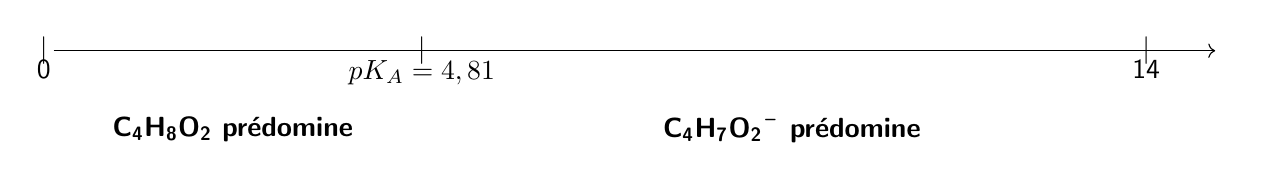
\begin{tikzpicture}
\node (O) at (0,0) {};
\node (A) at (4.8,0) {};
\node (B) at (14,0) {};
\node (F) at (15,0) {};
%\node (PredUp) at (3,.5) {$[AH]_{\text{éq}} > [A-]_{\text{éq}}$};
\node (PredDwn) at (2.4,-1) {\textbf{\ce{C4H8O2} prédomine}};
%\node (DomUp) at (9,.5) {$[AH]_{\text{éq}} < [A-]_{\text{éq}}$};
\node (DomDwn) at (9.5,-1) {\textbf{\ce{C4H7O2-} prédomine}};
\draw (O) node{$|$} node[below]{0};
\draw (A) node{$|$} node[below]{$pK_A=4,81$};
\draw (B) node{$|$} node[below]{14};
\draw[->] (O) to (F);
\end{tikzpicture}
\end{center}
	\item Le pH de l'estomac n'est pas constant. Lors d'une digestion idéale, il varie de 1,5 à 5. Préciser la ou les formes adoptées par l'espèce chimique lors de ces phases de digestion.\\
	\textcolor{blue}{Lors de la digestion, lorsque le pH est au plus bas, la forme acide butanoïque sera prédominante, mais lorsque le pH sera le plus élevé ce sera la forme butanoate qui sera prédominante. On notera qu'il existera une phase où les deux formes seront présentes de manière équivalentes aux alentours de la valeur du $pK_A$}
\end{enumerate}
\textbf{Donnée :} $pK_A$ du couple acide-base : $pK_A$ = 4,81

\section*{Exercice 5 : Acide phosphorique}
L'acide phosphorique est un triacide de formule \ce{H3PO4}. Les valeurs des trois $pK_A$ sont : 2,15 ; 7,20 et 12,3.
\begin{enumerate}
	\item Écrire les trois couples acide-base correspondant\\
	\textcolor{blue}{Les trois couples sont :\\
	\ce{H3PO4}/\ce{H2PO4-}\\
	\ce{H2PO4-}/\ce{HPO4^{2-}}\\
	\ce{HPO4^{2-}}/\ce{PO4^{3-}}}
	\item Représenter le diagramme de prédominance\\
\begin{center}
	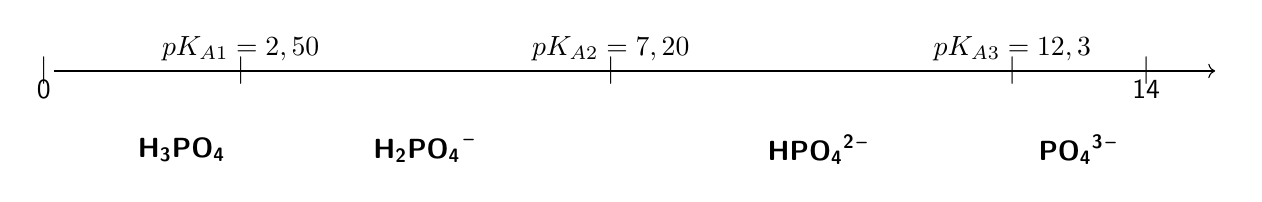
\begin{tikzpicture}
\node (O) at (0,0) {};
\node (A) at (2.5,0) {};
\node (AB) at (7.2,0) {};
\node (AC) at (12.3,0) {};
\node (B) at (14,0) {};
\node (F) at (15,0) {};
\node (ADwn) at (1.75,-1) {\textbf{\ce{H3PO4}}};
\node (ABDwn) at (4.85,-1) {\textbf{\ce{H2PO4-}}};
\node (ACDwn) at (9.85,-1) {\textbf{\ce{HPO4^{2-}}}};
\node (ABDwn) at (13.15,-1) {\textbf{\ce{PO4^{3-}}}};
\draw (O) node{$|$} node[below]{0};
\draw (A) node{$|$} node[above]{$pK_{A1}=2,50$};
\draw (AB) node{$|$} node[above]{$pK_{A2}=7,20$};
\draw (AC) node{$|$} node[above]{$pK_{A3}=12,3$};
\draw (B) node{$|$} node[below]{14};
\draw[->] (O) to (F);
\end{tikzpicture}
\end{center}
	\item L'acide phosphorique est-il un acide fort ?\\
	\textcolor{blue}{Un acide fort est un acide dont la dissociation est considérée comme totale, c'est à dire qu'il présente une constante d'équilibre supérieure à $10^4$. Le $pK_{A1}$ de l'acide phosphorique vaut 2,50 soit une constante d'équilibre $K_A = 10^{-pK_A} = 10^{-2,50} =\num{3,16e-3}$. On note que la constante d'acidité est inférieure à $10^4$, donc il s'agit d'un acide faible.}
	\item Comment qualifier l'ion \ce{H2PO4-(aq)} ?\\
	\textcolor{blue}{L'ion \ce{H2PO4-} peut agir à la fois comme un acide dans le couple \ce{H2PO4-}/\ce{HPO4^{2-}} et comme une base dans le couple \ce{H3PO4}/\ce{H2PO4-}. Il s'agit donc d'un composé amphotère}
\end{enumerate}

\section*{Exercice 6 : Le cyanure}
L'ion cyanure est une base de formule \ce{CN-(aq)}. Les sels de cyanure ainsi que son acide conjugué sont très toxiques.
\begin{enumerate}
	\item Exprimer la constante d'acidité du couple\\
	\textcolor{blue}{La réaction a pour équation : \ce{CN-(aq) + H2O(l) <=> HCN(aq) + HO-(aq)}}
\end{enumerate}
On dispose de \num{50} \unit{\milli \liter} de solution à une concentration en soluté apporté $c$ = \num{0,020} \unit{\mole \per \liter}. le pH de la solution est égal à 10,7.
\begin{enumerate}
\setcounter{enumi}{1}
	\item Conclure quant à la force de la base\\
	\textcolor{blue}{Pour juger la force de la base, il faut avoir accès à sa constante de réaction avec l'eau. $K_B = \dfrac{[\ce{HCN}]_{eq} \cdot [\ce{HO-}]_{eq}}{[\ce{CN-}]_{eq}}$\\ Pour estimer la concentration en ions \ce{HO-} il faut utiliser le produit ionique de l'eau : $K_e = [\ce{HO-}]\cdot [\ce{H3O+}]$ donc $[\ce{HO-}]_{eq} = \dfrac{K_e}{[\ce{H3O+}]} = \dfrac{K_e}{10^{-pH}} = \dfrac{10^{-14}}{10^{-10,7}} =\num{5e-4}\unit{\mole\per\liter}$\\
	Il est ensuite possible de déduire $\ce{CN-}]_{eq}$ car $\ce{CN-}]_{eq}=c-[\ce{HO-}]_{eq} = \num{2e-2}-\num{5e-4} = \num{1,95e-2}\unit{\mole\per\liter}$\\
	Enfin la constante de réaction donne : $K_B = \dfrac{[\ce{HCN}]_{eq} \cdot [\ce{HO-}]_{eq}}{[\ce{CN-}]_{eq}} = \dfrac{(\num{5e-4})^2}{\num{1,95e-2}} = \num{1,3e-5}$. Il ne s'agit pas d'une base forte car la constante d'équilibre est trop faible.}
\end{enumerate}

\section*{Exercice 7 : Aspirine}
L'aspirine est un acide faible dans l'eau, aussi appelé acide acétylsalicylique et noté ici \ce{AH(aq)}. On dissout un comprimé qui contient $m$ = \num{500} \unit{\milli \gram} d'aspirine dans un verre d'eau de volume $V$ = \num{25} \unit{\centi \liter}.
\begin{enumerate}
	\item Déterminer la concentration $c$ en soluté apporté\\
	\textcolor{blue}{$c=\dfrac{m}{M\cdot V} = \dfrac{0,5}{180,2 \times 0,25} = \num{1,11e-2}\unit{\mole\per\liter}$}
	\item Écrire l'équation de la réaction de l'acide acétylsalicylique avec l'eau et en déduire l'expression de la constante d'acidité.\\
	\textcolor{blue}{Équation de la réaction : \ce{AH(aq) + H2O(l) <=> A-(aq) + H3O+(aq)}\\
	$K_A = \dfrac{[\ce{A-}]_{eq} \cdot [\ce{H3O+}]_{eq}}{[\ce{AH}]_{eq}}$}
	\item Le taux de dissociation d'une acide $\tau$ est défini comme le taux d'avancement de sa réaction avec l'eau : $\tau = \dfrac{x_f}{x_{max}}$.
	\begin{enumerate}
		\item Exprimer les concentrations $[\ce{AH}]_{\text{éq}}$, $[\ce{A-}]_{\text{éq}}$ et $[\ce{H3O+}]_{\text{éq}}$ en fonction de $c$ et $\tau$\\
		\textcolor{blue}{En utilisant un tableau d'avancement on peut déterminer que \fbox{$x_{max}=c \cdot V$} et que $x_f=c \cdot V - [\ce{AH}]_{eq}$ soit \fbox{$x_f=V(c-[\ce{AH}]_{eq})$}\\
		On peut alors exprimer $\tau$ comme étant : $\tau=\dfrac{V(c-[\ce{AH}]_{eq})}{c \cdot V}$ ce qui donne $\tau=\dfrac{c-[\ce{AH}]_{eq}}{c}$\\
		$[\ce{AH}]_{eq}$ peut s'écrire à partir  de l'expression précédente : \fbox{$[\ce{AH}]_{eq} =c(1-\tau)$}\\
		$[\ce{A-}]_{eq} = [\ce{H3O+}]_{eq}$ correspond à l'avancement final divisé par le volume soit $[\ce{A-}]_{eq}=\dfrac{x_f}{V}=\dfrac{V(c-[\ce{AH}]_{eq})}{V}=c-[\ce{AH}]_{eq}$. Comme $[\ce{AH}]_{eq} =c(1-\tau)$, on aura : $[\ce{A-}]_{eq}=c-c(1-\tau) = c\cdot\tau$.\\
		Au final on aura \fbox{$[\ce{A-}]_{eq} = [\ce{H3O+}]_{eq}=c\cdot\tau$}
		}
		\item Établir que le taux de dissociation peut être calculé en résolvant l'équation du second degré : $c \cdot \tau^2 + K_A \cdot \tau - K_A = 0$\\
		\textcolor{blue}{À partir des expressions précédentes, la constante d'équilibre peut s'écrire : $K_A = \dfrac{(c \cdot \tau)^2}{c(1-\tau)}$\\
		En transformant l'expression elle devient : $K_A \cdot c \cdot (1-\tau)=c^2\cdot\tau^2$\\
		En simplifiant et en distribuant elle devient : $K_A -K_A\cdot \tau = c\cdot \tau^2$\\
		Enfin en ramenant du même coté, l'équation suivante est obtenue : \fbox{$c \cdot \tau^2 + K_A \cdot \tau - K_A=0$}}
		\item Calculer $\tau$, puis le pH se la solution\\
		\textcolor{blue}{Pour calculer $\tau$, il faut résoudre l'équation précédente.\\
		Calcul du discriminant : $\Delta = b^2 - 4 \cdot a \cdot c = K_A^2 - 4 \cdot c \cdot (-K_A)$ \\
		\fbox{AN} : $(10^{-3,5})^2 + 4 \cdot \num{1,11e-2} \cdot (10^{-3,5}) = \num{1,41e-5}$\\
		Le discriminant est positif, il existe donc deux solutions réelles : $\tau_1 = \dfrac{-K_A-\sqrt{\Delta}}{2\cdot c} \text{ et } \tau_2 = \dfrac{-K_A+\sqrt{\Delta}}{2\cdot c}$\\
		\fbox{AN} : $\tau_1 = \dfrac{-10^{-3,5}-\sqrt{\num{1,41e-5}}}{2\cdot \num{1,11e-2}} \text{ et } \tau_2 = \dfrac{-10^{-3,5}+\sqrt{\num{1,41e-5}}}{2\cdot \num{1,11e-2}}$\\
		$\tau_1 = \num{1,84e-1} \text{ et } \tau_2 = \num{1,55e-1}$\\
		Le taux d'avancement positif sera celui retenu donc \fbox{$\tau = 0,15$}\\
		Le pH est accessible par la concentration en ions \ce{H3O+}, on a : $[\ce{H3O+}]_{eq}=c\cdot\tau$ donc $pH = -log(c\cdot\tau)$ \\
		\fbox{AN} : $pH = -log(\num{1,11e-2} \times 0,15)=2,8$}
		\item Déterminer la forme sous laquelle se trouve l'acide acétylsalicylique dans le verre\\
		\textcolor{blue}{Le pH de la solution est inférieur à la valeur de $pK_A$ c'est donc l'acide AH qui prédomine.}
	\end{enumerate}
\end{enumerate}
\textbf{Données :}
\begin{itemize}
	\item Masse molaire de l'aspirine : $M$ = \num{180,2} \unit{\gram \per \mole}
	\item $pK_A$ du couple considéré : $pK_A$ = 3,5 
\end{itemize}

\section*{Exercice 8 : Indicateur coloré}
Un flacon opaque d'un indicateur coloré est découvert, avec pour seules indications sa concentration en quantité de matière $c$ = \num{2,90e-4} \unit{\mole \per \liter} et son pH de 4,18. Le couple acide-base se cet indicateur coloré sera noté \ce{HInd}/\ce{Ind-}
\begin{enumerate}
	\item Déterminer la concentration en ion oxonium
	\item Déterminer le taux d'avancement de la réaction entre la forme \ce{HInd} et l'eau
	\item Établir que la constante d'acidité de l'indicateur coloré vaut $K_A$ = \num{1,9e-5}
	\item Identifier l'indicateur coloré retrouvé et la couleur de la solution à l'aide du tableau suivant.
\end{enumerate}
\begin{tabular}{|>{\centering}m{3.5cm}|>{\centering}m{3.5cm}|>{\centering}m{3.5cm}|>{\centering}m{3.5cm}|>{\centering\arraybackslash}m{3.5cm}|}
\hline Indicateur & Couleur acide & Zone de virage & Couleur basique & $pK_A$\\
\hline Héliantine & Rouge & 3,2 - 4,4 & Jaune orangé & 3,7\\
\hline Vert de bromocrésol & Jaune & 3,8 - 5,4 & Bleu & 4,7\\
\hline Bleu de bromocrésol & Jaune & 6,0 - 7,6 & Bleu & 7,0\\
\hline
\end{tabular}

\section*{Exercice 9 : Arc-en-ciel végétal}
Certaines fleurs possèdent des pigments naturels dont la couleur dépend du pH. la couleur violette est due à une molécule amphotère que l'on note \ce{AH(aq)}.
\begin{enumerate}
	\item Écrire l'équation de la réaction de \ce{AH(aq)} en tant qu'acide avec l'eau
	\item Donner l'expression de la constante d'équilibre $K_{A2}$ de cette réaction, puis la calculer
	\item Le pH d'une solution contenant \ce{AH(aq)} est égal à 10. Exprimer littéralement le rapport $\dfrac{[\ce{A-}]_{\text{éq}}}{[\ce{AH}]_{\text{éq}}}$ et en déduire la couleur de la solution
	\item Écrire l'équation de la réaction de \ce{AH(aq)} en tant que base avec l'eau.
	\item Donner l'expression de la constante d'équilibre de la réaction en fonction de $K_{A1}$
	\item Réaliser le diagramme de prédominance des espèces \ce{AH2+(aq)}, \ce{AH(aq)} et \ce{A-(aq)}
	\item Déterminer le domaine de pH pour lequel la molécule est bleue
\end{enumerate}
\textbf{Données :}
\begin{itemize}
	\item $pK_A$ des espèces colorées : $pK_{A1}$ = 4,3 et $pK_{A2}$ = 7,0
	\item Couleur de \ce{AH2+(aq)} : rouge
	\item Couleur de \ce{AH(aq)} : violette
	\item Couleur de \ce{A-(aq)} : bleue
\end{itemize}

\section*{Exercice 10 : Détermination d'un $pK_A$}
On souhaite déterminer expérimentalement le $pK_A$ d'un couple acide-base. Pour cela, on considère une solution placée dans le domaine de prédominance de l'acide. On suppose que la quantité de base est négligeable, et on note $n_0$ la quantité de matière de l'acide. À l'aide d'une burette, on ajoute progressivement une solution de soude (\ce{Na+(aq)} ; \ce{HO-(aq)}) et on mesure le pH de la solution au fur et à mesure. On notera $c_{soude}$ la concentration de la solution de soude.
\begin{enumerate}
	\item Écrire l'équation de la réaction ayant lieu\\
	\textcolor{blue}{\ce{AH(aq) + HO-(aq) -> A-(aq) + H2O(l)}}
	\item À quel montage correspond cette expérience ?\\
	\textcolor{blue}{Il s'agit d'un titrage de l'acide \ce{AH(aq)} par une base forte (la soude).}
	\item Comment repère-t-on le moment où les réactifs ont été introduits dans les proportions stœchiométriques ? On note $V_E$ le volume de soude versé correspondant.\\
	\textcolor{blue}{Le moment où les réactifs sont introduits en proportions stœchiométriques correspond à un changement important dans la valeur du pH : tout l'acide AH présent est consommé et la quantité d'ions \ce{H3O+(aq)} diminue rapidement avec l'ajout de petites quantités de soude. Il en résulte un "saut" dans les valeurs de pH observées sur la courbe. On appelle cet instant l'équivalence et il est accessible par lecture graphique au moyen de la méthode des tangentes}
	\item Écrire une relation vérifiée entre $V_E$, $c_{soude}$ et $n_0$\\
	\textcolor{blue}{À l'équivalence on a : $n_{\ce{AH}} = n_{\ce{HO-}}$ soit $n_0 = c_{soude} \cdot V_E$}
	\item La courbe obtenue pour le couple de l'acide éthanoïque \ce{C2H4O2(aq)}/\ce{C2H3O2-(aq)}. Déterminer le $pK_A$ de ce couple\\
	\textcolor{blue}{À l'équivalence, c'est la totalité \ce{AH(aq)} qui est consommée par les ions \ce{HO-(aq)} versés. Or le $pK_A$ correspond à l'équilibre pour lequel les quantités de \ce{AH} et \ce{A-} sont équivalentes. On peut alors dire que le $pK_A$ est atteint à la moitié vu volume de soude versé avant d'atteindre l'équivalence. On peut donc déterminer graphiquement le $pK_A$.\\ On a un volume équivalent de 13,3 mL.}
\end{enumerate}

\includegraphics[scale=.8]{TSPE_C8_Exercices_Fig1b.png
}
\end{document}